\documentclass[10pt,twocolumn,letterpaper]{article}


\usepackage{todonotes}
\usepackage{cvpr}
\usepackage{times}
\usepackage{epsfig}
\usepackage{graphicx}
\usepackage{amsmath}
\usepackage{amssymb}
\usepackage{enumitem}
\usepackage{subcaption}

\usepackage[backend=biber]{biblatex}


% Include other packages here, before hyperref.

% If you comment hyperref and then uncomment it, you should delete
% egpaper.aux before re-running latex.  (Or just hit 'q' on the first latex
% run, let it finish, and you should be clear).
\usepackage[breaklinks=true,bookmarks=false]{hyperref}

\cvprfinalcopy % *** Uncomment this line for the final submission

\def\cvprPaperID{****} % *** Enter the CVPR Paper ID here
\def\httilde{\mbox{\tt\raisebox{-.5ex}{\symbol{126}}}}
\bibliography{bibliography}
% Pages are numbered in submission mode, and unnumbered in camera-ready
%\ifcvprfinal\pagestyle{empty}\fi
%\setcounter{page}{4321}
\begin{document}

%%%%%%%%% TITLE
\title{Report: Practical to Advanced Deep Learning in Computer Vision}

\author{Alexander Ziller\\
%Institution1\\
%Institution1 address\\
{\tt\small alex.ziller@tum.de}
% For a paper whose authors are all at the same institution,
% omit the following lines up until the closing ``}''.
% Additional authors and addresses can be added with ``\and'',
% just like the second author.
% To save space, use either the email address or home page, not both
\and
Leonhard Feiner\\
%Institution2\\
%First line of institution2 address\\
{\tt\small leo.feiner@tum.de}
}

\maketitle
%\thispagestyle{empty}

%%%%%%%%% ABSTRACT
\begin{abstract}
During the practical we have been working on improving pose regression networks accuracy by multi-task learning with semantic information. In this final report we are shortly reporting our approaches and results. We could show that multi-task learning outperforms state-of-the-art pose regression methods without semantic information. Yet it does not outperform the more complex architecture of Radwan et al.
\end{abstract}

%%%%%%%%% BODY TEXT
\section{Introduction}
\subsection{Problem formulation}
Radwan et al \cite{radwan18ral} showed that semantic information can improve pose estimation i.e. estimating location and rotation of a given image from a scene. Our task was to see whether a simpler architecture could also profit from this. 
\subsection{Baseline approaches}
\subsubsection{Mapnet}\label{sec:mapnet}
As baseline for our pose estimation results we are using Mapnet\cite{mapnet2018}. Mapnet uses a pretrained ResNet-34 as a feature extraction network and afterwards several linear layers to regress a six dimensional pose vector (see grey part in Figure \ref{fig:arch}). Note that we are not comparing to MapNet++, which includes GPS and VO data.
\subsubsection{Segmentation network}\label{sec:segnet}
To test whether multi-task learning of poses and semantics also boosts the latter we implemented a model which uses a ResNet-34 as feature extraction network and afterwards several upsampling layers with skip connections from the feature extraction layers. This was inspired by the famous U-Net paper\cite{ronneberger2015u}. Note that this architecture was also used in the multi-task model. 
\subsection{Dataset}\label{sec:data}
We are using the DeepLoc dataset\cite{radwan18ral}. It includes a training and validation set each consisting of stereo RGB images, depth data and semantic information for every second datapoint. 

\section{Our approaches}
\begin{figure}[t]
	\begin{center}
		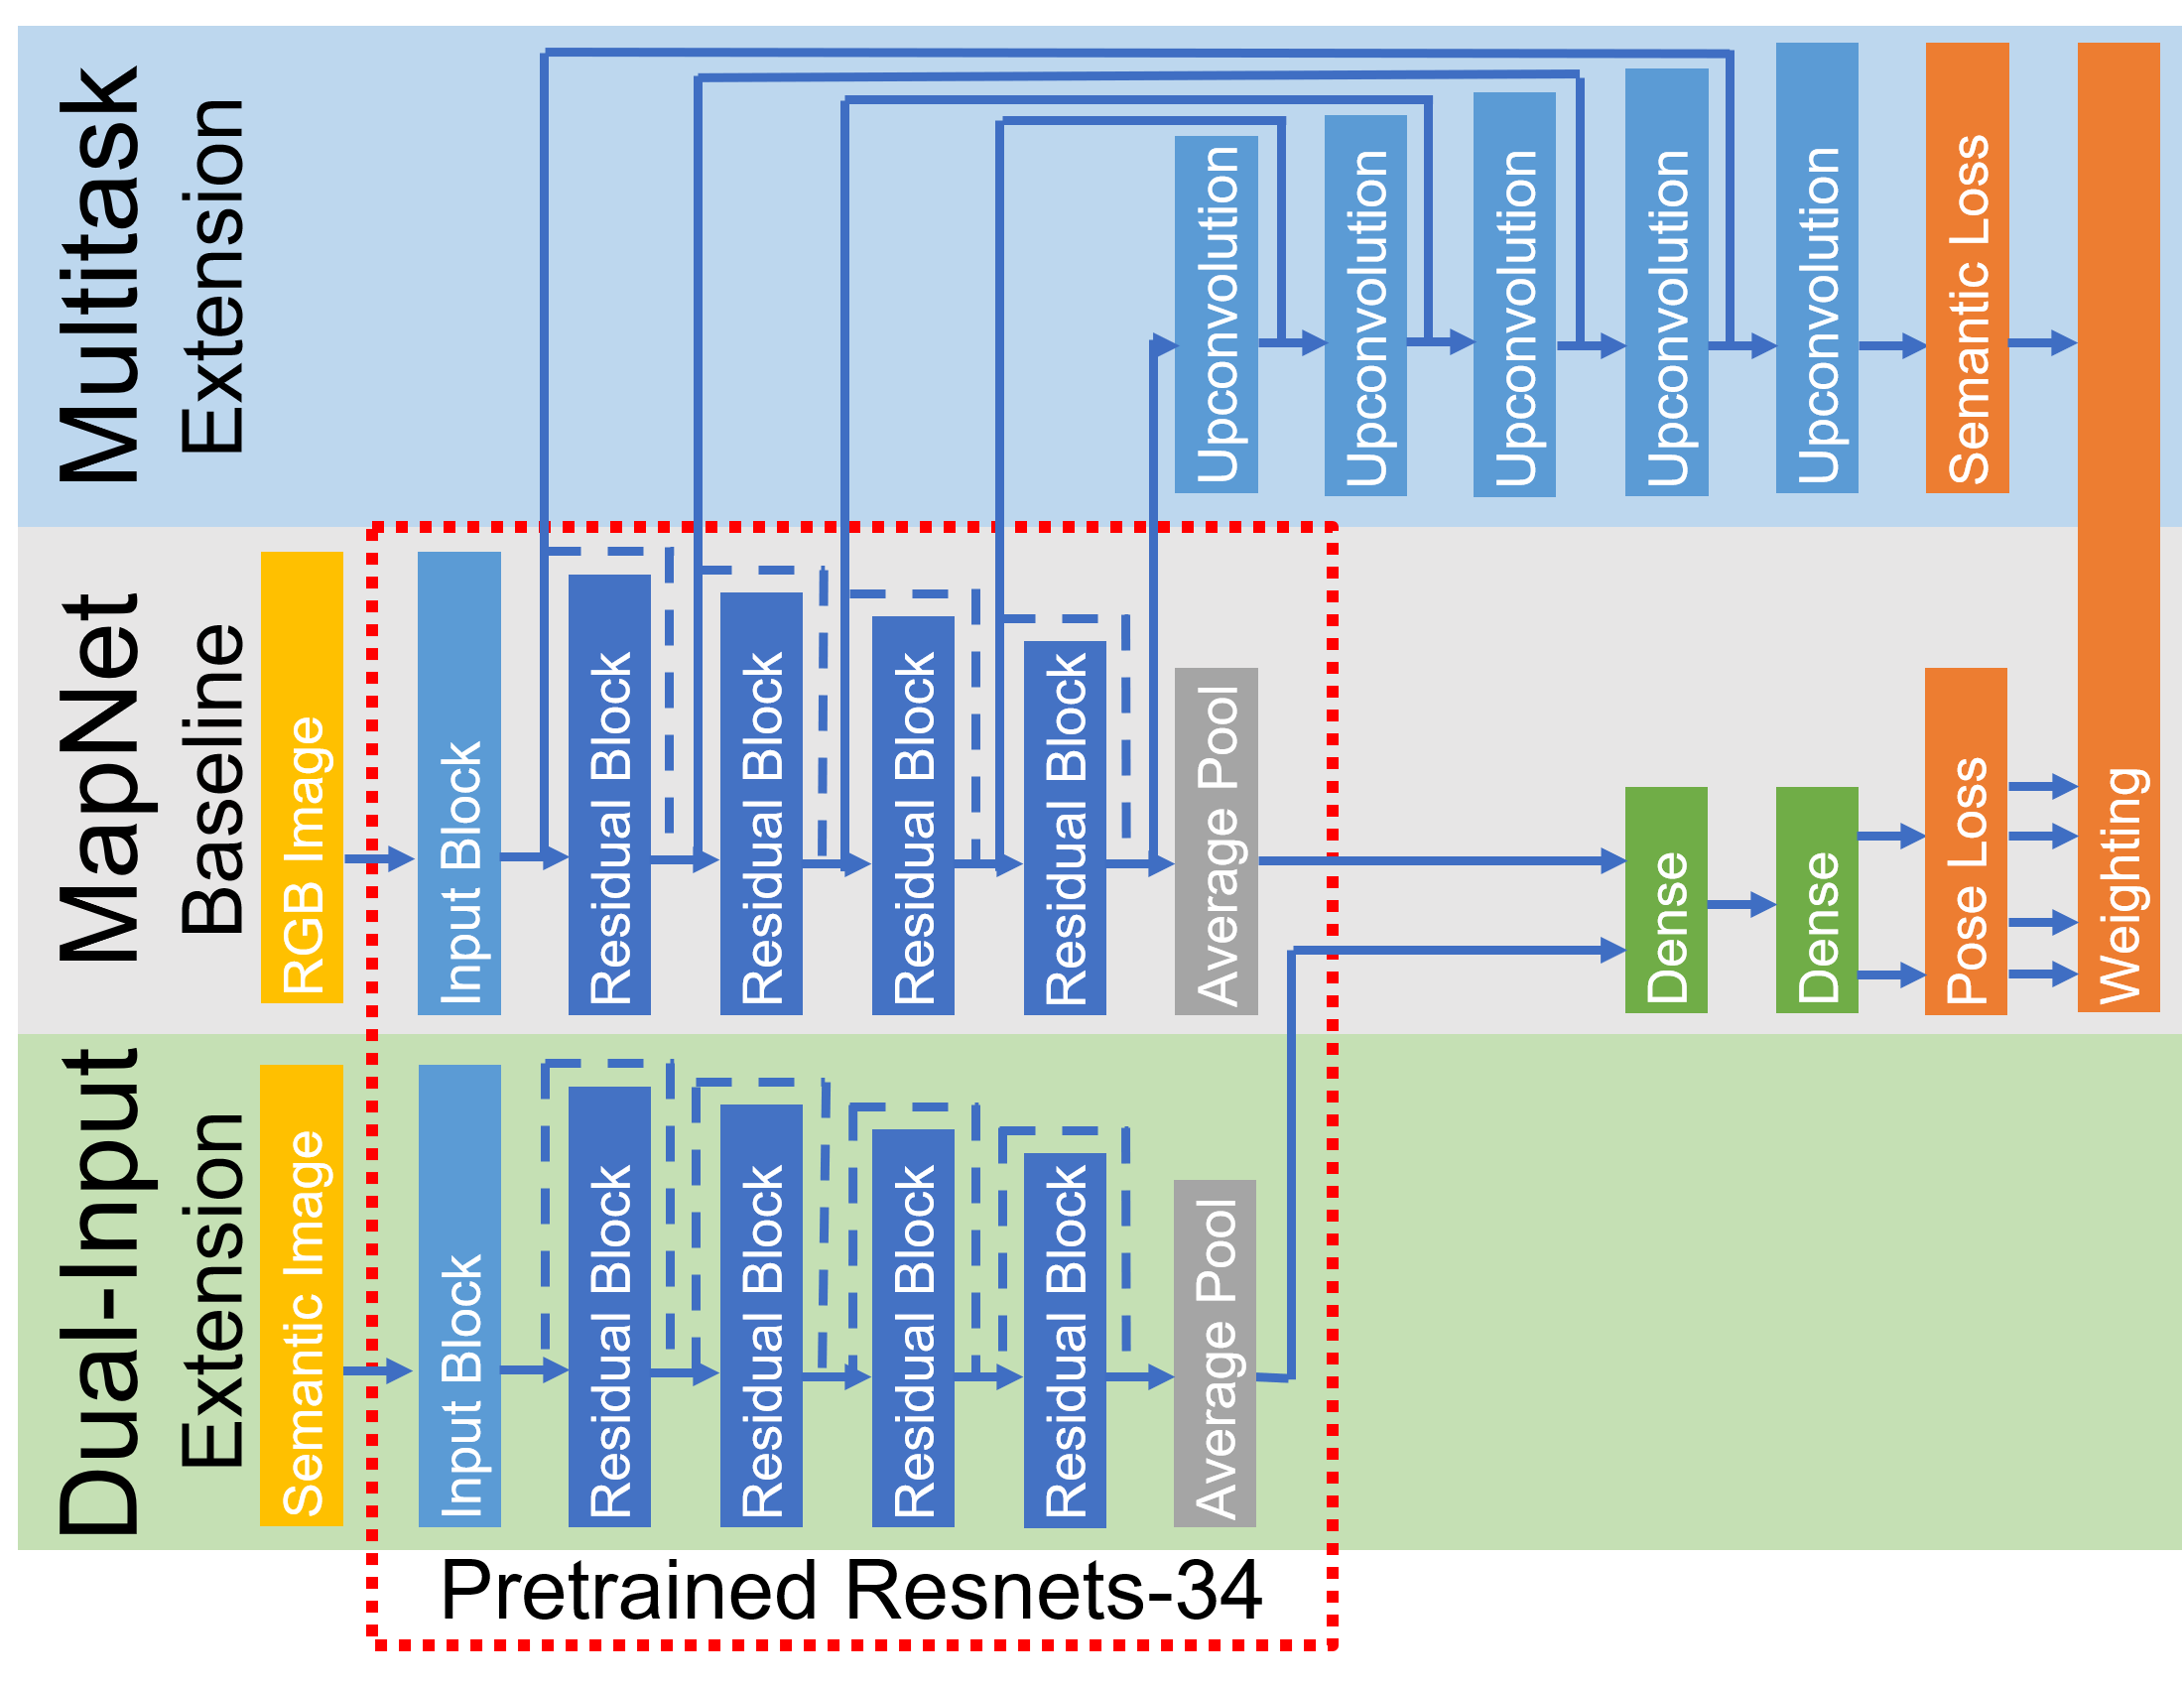
\includegraphics[width=0.8\linewidth]{images/architektur.png}
	\end{center}
	\caption{Visualization of architectures (grey: MapNet, green+grey: Dual-Input model, blue: segmentation network, grey+blue: Multi-task model)}
	\label{fig:arch}
\end{figure}
\subsection{Dual input model}\label{sec:dualinput}
The simplest approach to test if semantic information could boost pose estimation is to feed it as additional input to the network (see green part of Figure \ref{fig:arch}). Because the input data has ten input channels we could not use a pretrained feature extraction network, which has three input channels for RGB data, naively. 
%We implemented several versions for this approach. One was to convert semantic information to a RGB image like it is done for visualization and feed it to the feature extraction network. For the other version we extracted an additional fourth channel for the feature extraction initialized by the average of the other channel's weights. 
We implemented and tested several approaches to solve this problem. Most of them were based on the idea to convert labels to RGB data as it is done in visualization and feed it then to the network. The other idea was to bring it to one channel and create a fourth input layer for the feature extraction network by using the average weights of the other three pretrained layers. 
Empirically it showed that the conversion to RGB data without shared weights in the feature extraction part gives best results and therefore is considered in the following as Dual input model.
%\missingfigure{Model architecture}
\subsection{Multi-task model}\label{sec:multitask}
This model is a fusion of MapNet from \ref{sec:mapnet} and the segmentation network described in \ref{sec:segnet} (see Figure \ref{fig:arch}). It takes a RGB image as input and outputs semantic segmentation and a pose estimation. The weighting of Losses is essential to performance and is described in \ref{sec:losses}
\subsection{Loss formulation}\label{sec:losses}
The loss is comprised of different individual loss terms, measuring performance on absolute and relative translation and rotation output. 
\begin{align}
\mathcal{L}^{combined} &=\mathcal{L}^{weighted}_{trans,abs}+ \mathcal{L}^{weighted}_{rot,abs}+\mathcal{L}^{weighted}_{trans,rel}+\mathcal{L}^{weighted}_{rot,rel}
\end{align}
Each of these individual losses is weighted. For MapNet and Dual input model this is according to the geometric weighting of the MapNet paper \cite{mapnet2018}.
In the following equations we use $X$ as $X \in \{(trans,abs);(trans,rel);(rot,abs);(rot,rel)\}$.
\begin{align}
\mathcal{L}^{weighted}_X &= e^{-\alpha_X}\mathcal{L}_X +\alpha_X
\end{align}

For Multi-task the losses are combined by a learned weighting as described in \cite{kendall2018multi}. 
\begin{align}
\mathcal{L}^{weighted}_X &= \frac{1}{2\sigma^2_X}\mathcal{L}_X+\log(\sigma_X)\\
\mathcal{L}^{weighted}_{semantics} &= \frac{1}{\sigma^2_X}\mathcal{L}_X+\log(\sigma_X)
\end{align}
In these Loss terms $\alpha$ and $\log(\sigma)$ are learnable weights.
%\missingfigure{Multitask architecture}
\section{Results}
\subsection{Pose estimation errors}
To evaluate pose estimation we calculate mean and median of translation and rotation error on validation data. We also compare it to results given in \cite{radwan18ral} which used the same dataset. See Figure \ref{fig:pose_graphs} for visualization of pose estimation errors.
\begin{tabular}{ll||l|l|l|l}
	Model&Source&median&mean&median&mean\\\hline
	PoseNet & Our &3.64m &4.44m&3.13$^\circ$ &	4.27$^\circ$ \\
	PoseNet & \cite{radwan18ral} &2.42m &&3.66$^\circ$&\\
	MapNet & Our &3.42m &3.91m &3.23$^\circ$&4.48$^\circ$\\
	Dual-Input & Our &3.26m&3.54m&2.82$^\circ$&4.32$^\circ$\\
	Mult-task & Our &1.07m&1.31m&2.96$^\circ$&4.32$^\circ$\\
	VlocNet & \cite{radwan18ral} &0.68m&&3.43$^\circ$&\\
	VlocNet++ & \cite{radwan18ral} &0.37m&&1.93$^\circ$&
\end{tabular}
%\missingfigure{Pose graphs}
\begin{figure}[t]
	\begin{center}
		\begin{subfigure}{.23\textwidth}
		\begin{center}
			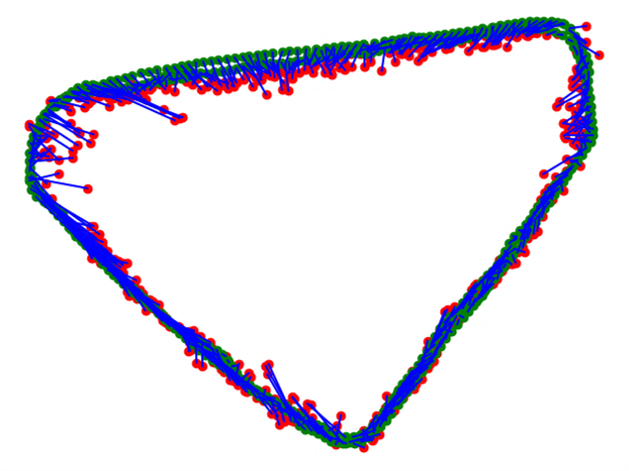
\includegraphics[width=0.8\linewidth]{images/posenet.png}
			\caption{PoseNet}
		\end{center}
	\end{subfigure}
	\begin{subfigure}{.23\textwidth}
		\begin{center}
			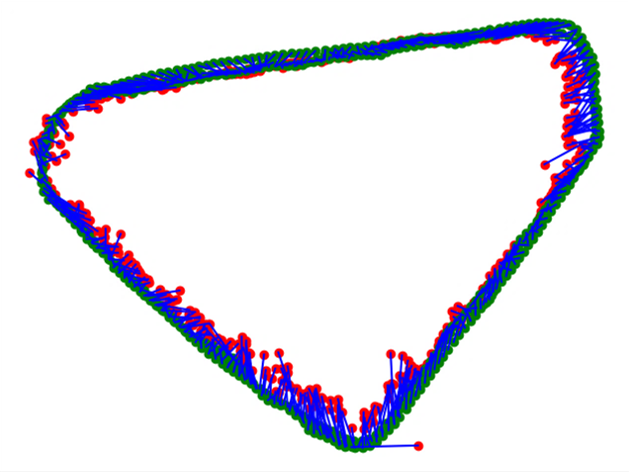
\includegraphics[width=0.8\linewidth]{images/mapnet.png}
			\caption{MapNet}
		\end{center}
	\end{subfigure}
\begin{subfigure}{.23\textwidth}
\begin{center}
	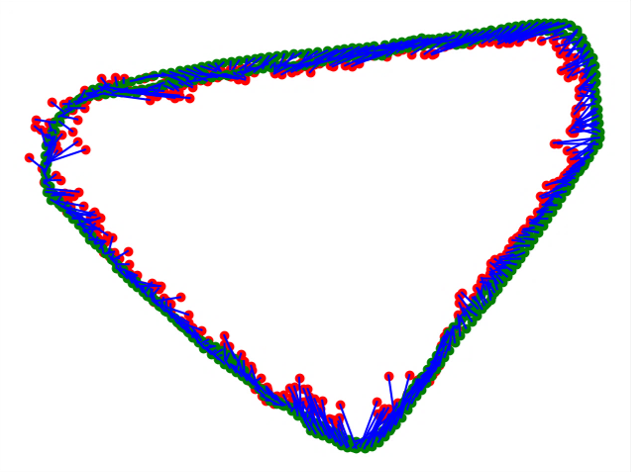
\includegraphics[width=0.8\linewidth]{images/dualinput.png}
	\caption{Dual Input}
\end{center}
\end{subfigure}
	\begin{subfigure}{.23\textwidth}
	\begin{center}
		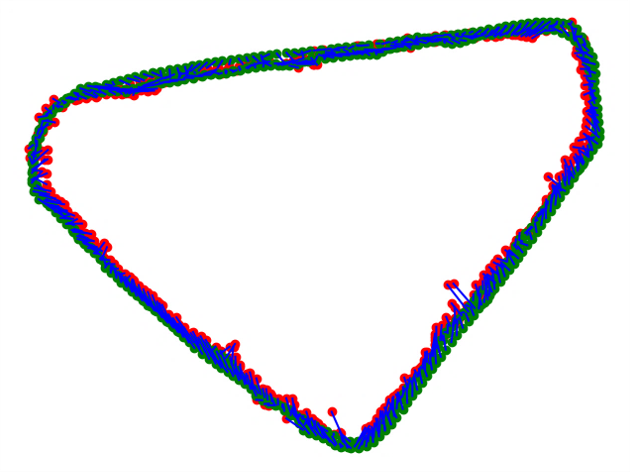
\includegraphics[width=0.8\linewidth]{images/multitask.png}
		\caption{Multi-task}
	\end{center}
\end{subfigure}
\end{center}

	\caption{Pose graphs on validation data. Green dots: Ground truth; Red dots: Predicted points; Blue lines: Connecting corresponding dots}
	\label{fig:pose_graphs}
\end{figure}
\subsection{Segmentation results}
Both segmentation and mult-task model reach a pixel accuracy of 96\%. The difference is too low to conclude that one of these methods is better i.e. on this dataset pose regression did not boost segmentation results significantly.
\begin{figure}[t]
	\begin{center}
		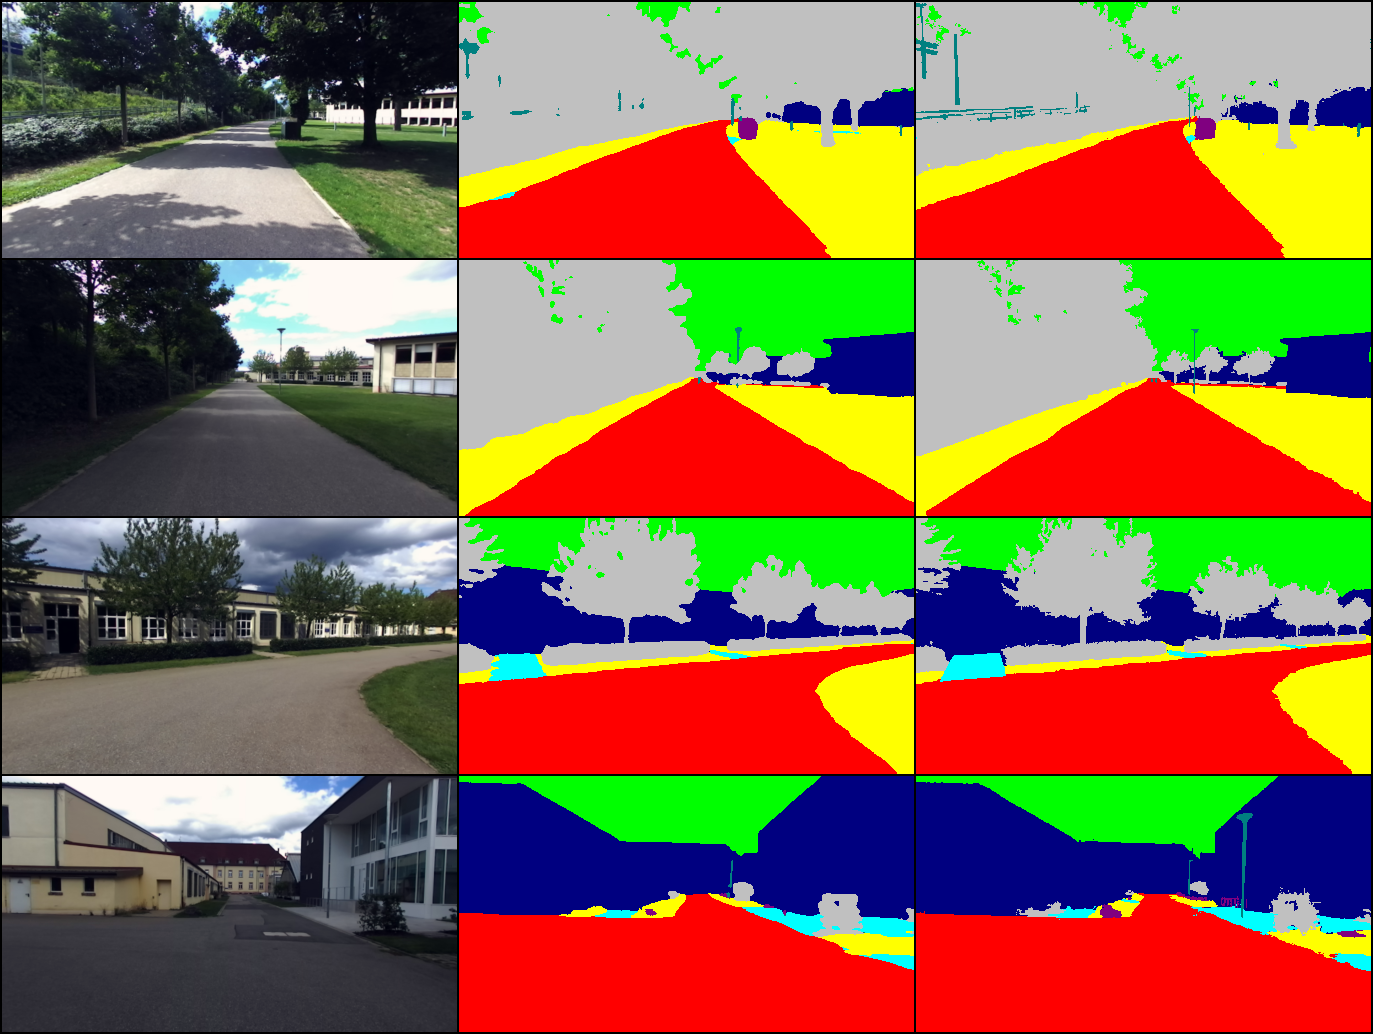
\includegraphics[width=0.8\linewidth]{images/semantic_results_semanticOutput.png}
	\end{center}
	\caption{Semantic segmentation input, result and target for validation data}
	\label{fig:sem_seg}
\end{figure}

\section{Challenges}
Throughout the practical we faced several challenges. Some of them should be mentioned as they are critical to training and evaluation. 
\begin{itemize}[noitemsep,topsep=1pt]
	\item Dataset does not contain test set. We used validation data as test data. Bad practice but ensures comparability to other papers.
	\item Only every second image has semantic ground truth.
	\item Random initialization influences results significantly.
	\item Dataset had error in groundtruth until January.
\end{itemize}

\subsection{Attention visualization}
To make it more visual which features the network is interested in we implemented the visualization technique from \cite{chattopadhay2018grad}. See Figure \ref{fig:attention_map}.
\begin{figure}[t]
\begin{center}
   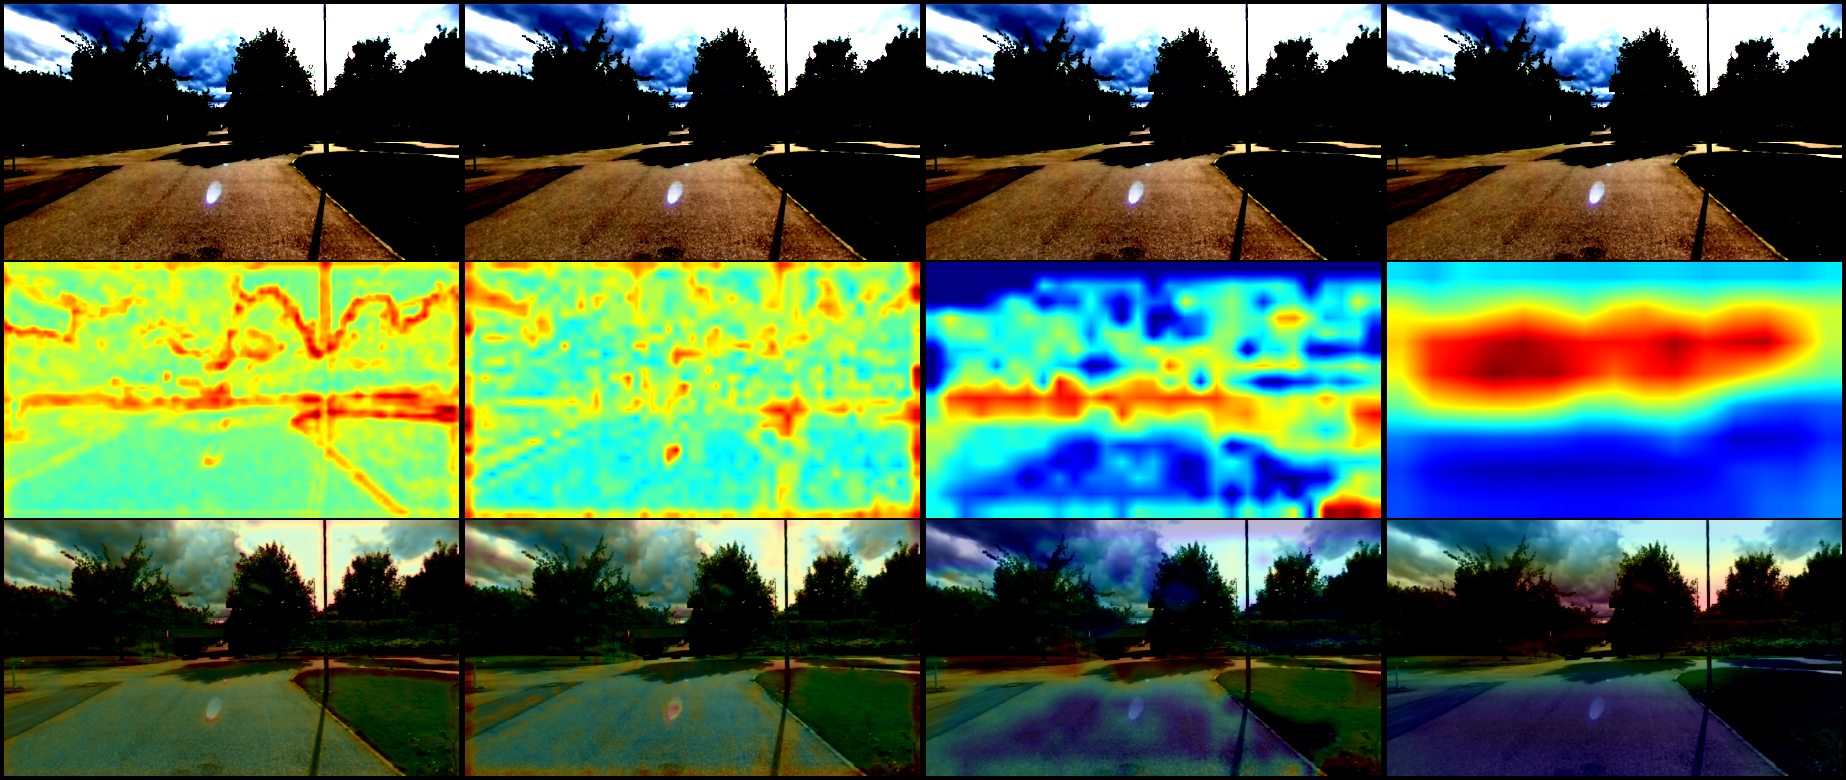
\includegraphics[width=0.8\linewidth]{images/activation_maps_multitask_layer1,layer2,layer3,layer4.png}
\end{center}
   \caption{Backpropagated attention in layers 1 to 4 of the feature extraction network.}
\label{fig:attention_map}
\end{figure}

\section{Conclusion}
Overall we can conclude that multi-task learning is a simple and light weight way to improve pose estimation with neural networks. However, our model was not able to compete with VLocNet++, which is using a more complex architecture and more input signals such as GPS and visual odometry.

\section*{Code references}
We used external code from following ressources:
\begin{itemize}[nosep,topsep=1pt]
\item 
Base repository:\\
\url{https://github.com/NVlabs/geomapnet}
\item 
Utils to calculate IoU for semantic segmentation:\\
\url{https://github.com/CSAILVision/semantic-segmentation-pytorch/blob/master/utils.py}
\item 
Calculation of attention maps:\\
\url{https://github.com/1Konny/gradcam_plus_plus-pytorch/blob/master/gradcam.py}
\end{itemize}
%
%
%%-------------------------------------------------------------------------
%\subsection{Language}
%
%All manuscripts must be in English.
%
%\subsection{Dual submission}
%
%Please refer to the author guidelines on the CVPR 2019 web page for a
%discussion of the policy on dual submissions.
%
%\subsection{Paper length}
%Papers, excluding the references section,
%must be no longer than eight pages in length. The references section
%will not be included in the page count, and there is no limit on the
%length of the references section. For example, a paper of eight pages
%with two pages of references would have a total length of 10 pages.
%{\bf There will be no extra page charges for CVPR 2019.}
%
%Overlength papers will simply not be reviewed.  This includes papers
%where the margins and formatting are deemed to have been significantly
%altered from those laid down by this style guide.  Note that this
%\LaTeX\ guide already sets figure captions and references in a smaller font.
%The reason such papers will not be reviewed is that there is no provision for
%supervised revisions of manuscripts.  The reviewing process cannot determine
%the suitability of the paper for presentation in eight pages if it is
%reviewed in eleven.  
%
%%-------------------------------------------------------------------------
%\subsection{The ruler}
%The \LaTeX\ style defines a printed ruler which should be present in the
%version submitted for review.  The ruler is provided in order that
%reviewers may comment on particular lines in the paper without
%circumlocution.  If you are preparing a document using a non-\LaTeX\
%document preparation system, please arrange for an equivalent ruler to
%appear on the final output pages.  The presence or absence of the ruler
%should not change the appearance of any other content on the page.  The
%camera ready copy should not contain a ruler. (\LaTeX\ users may uncomment
%the \verb'\cvprfinalcopy' command in the document preamble.)  Reviewers:
%note that the ruler measurements do not align well with lines in the paper
%--- this turns out to be very difficult to do well when the paper contains
%many figures and equations, and, when done, looks ugly.  Just use fractional
%references (e.g.\ this line is $095.5$), although in most cases one would
%expect that the approximate location will be adequate.
%
%\subsection{Mathematics}
%
%Please number all of your sections and displayed equations.  It is
%important for readers to be able to refer to any particular equation.  Just
%because you didn't refer to it in the text doesn't mean some future reader
%might not need to refer to it.  It is cumbersome to have to use
%circumlocutions like ``the equation second from the top of page 3 column
%1''.  (Note that the ruler will not be present in the final copy, so is not
%an alternative to equation numbers).  All authors will benefit from reading
%Mermin's description of how to write mathematics:
%\url{http://www.pamitc.org/documents/mermin.pdf}.
%
%
%\subsection{Blind review}
%
%Many authors misunderstand the concept of anonymizing for blind
%review.  Blind review does not mean that one must remove
%citations to one's own work---in fact it is often impossible to
%review a paper unless the previous citations are known and
%available.
%
%Blind review means that you do not use the words ``my'' or ``our''
%when citing previous work.  That is all.  (But see below for
%techreports.)
%
%Saying ``this builds on the work of Lucy Smith [1]'' does not say
%that you are Lucy Smith; it says that you are building on her
%work.  If you are Smith and Jones, do not say ``as we show in
%[7]'', say ``as Smith and Jones show in [7]'' and at the end of the
%paper, include reference 7 as you would any other cited work.
%
%An example of a bad paper just asking to be rejected:
%\begin{quote}
%\begin{center}
%    An analysis of the frobnicatable foo filter.
%\end{center}
%
%   In this paper we present a performance analysis of our
%   previous paper [1], and show it to be inferior to all
%   previously known methods.  Why the previous paper was
%   accepted without this analysis is beyond me.
%
%   [1] Removed for blind review
%\end{quote}
%
%
%An example of an acceptable paper:
%
%\begin{quote}
%\begin{center}
%     An analysis of the frobnicatable foo filter.
%\end{center}
%
%   In this paper we present a performance analysis of the
%   paper of Smith \etal [1], and show it to be inferior to
%   all previously known methods.  Why the previous paper
%   was accepted without this analysis is beyond me.
%
%   [1] Smith, L and Jones, C. ``The frobnicatable foo
%   filter, a fundamental contribution to human knowledge''.
%   Nature 381(12), 1-213.
%\end{quote}
%
%If you are making a submission to another conference at the same time,
%which covers similar or overlapping material, you may need to refer to that
%submission in order to explain the differences, just as you would if you
%had previously published related work.  In such cases, include the
%anonymized parallel submission~\cite{Authors14} as additional material and
%cite it as
%\begin{quote}
%[1] Authors. ``The frobnicatable foo filter'', F\&G 2014 Submission ID 324,
%Supplied as additional material {\tt fg324.pdf}.
%\end{quote}
%
%Finally, you may feel you need to tell the reader that more details can be
%found elsewhere, and refer them to a technical report.  For conference
%submissions, the paper must stand on its own, and not {\em require} the
%reviewer to go to a techreport for further details.  Thus, you may say in
%the body of the paper ``further details may be found
%in~\cite{Authors14b}''.  Then submit the techreport as additional material.
%Again, you may not assume the reviewers will read this material.
%
%Sometimes your paper is about a problem which you tested using a tool which
%is widely known to be restricted to a single institution.  For example,
%let's say it's 1969, you have solved a key problem on the Apollo lander,
%and you believe that the CVPR70 audience would like to hear about your
%solution.  The work is a development of your celebrated 1968 paper entitled
%``Zero-g frobnication: How being the only people in the world with access to
%the Apollo lander source code makes us a wow at parties'', by Zeus \etal.
%
%You can handle this paper like any other.  Don't write ``We show how to
%improve our previous work [Anonymous, 1968].  This time we tested the
%algorithm on a lunar lander [name of lander removed for blind review]''.
%That would be silly, and would immediately identify the authors. Instead
%write the following:
%\begin{quotation}
%\noindent
%   We describe a system for zero-g frobnication.  This
%   system is new because it handles the following cases:
%   A, B.  Previous systems [Zeus et al. 1968] didn't
%   handle case B properly.  Ours handles it by including
%   a foo term in the bar integral.
%
%   ...
%
%   The proposed system was integrated with the Apollo
%   lunar lander, and went all the way to the moon, don't
%   you know.  It displayed the following behaviours
%   which show how well we solved cases A and B: ...
%\end{quotation}
%As you can see, the above text follows standard scientific convention,
%reads better than the first version, and does not explicitly name you as
%the authors.  A reviewer might think it likely that the new paper was
%written by Zeus \etal, but cannot make any decision based on that guess.
%He or she would have to be sure that no other authors could have been
%contracted to solve problem B.
%\medskip
%
%\noindent
%FAQ\medskip\\
%{\bf Q:} Are acknowledgements OK?\\
%{\bf A:} No.  Leave them for the final copy.\medskip\\
%{\bf Q:} How do I cite my results reported in open challenges?
%{\bf A:} To conform with the double blind review policy, you can report results of other challenge participants together with your results in your paper. For your results, however, you should not identify yourself and should not mention your participation in the challenge. Instead present your results referring to the method proposed in your paper and draw conclusions based on the experimental comparison to other results.\medskip\\
%
%
%
%\begin{figure}[t]
%\begin{center}
%\fbox{\rule{0pt}{2in} \rule{0.9\linewidth}{0pt}}
%   %\includegraphics[width=0.8\linewidth]{egfigure.eps}
%\end{center}
%   \caption{Example of caption.  It is set in Roman so that mathematics
%   (always set in Roman: $B \sin A = A \sin B$) may be included without an
%   ugly clash.}
%\label{fig:long}
%\label{fig:onecol}
%\end{figure}
%
%\subsection{Miscellaneous}
%
%\noindent
%Compare the following:\\
%\begin{tabular}{ll}
% \verb'$conf_a$' &  $conf_a$ \\
% \verb'$\mathit{conf}_a$' & $\mathit{conf}_a$
%\end{tabular}\\
%See The \TeX book, p165.
%
%The space after \eg, meaning ``for example'', should not be a
%sentence-ending space. So \eg is correct, {\em e.g.} is not.  The provided
%\verb'\eg' macro takes care of this.
%
%When citing a multi-author paper, you may save space by using ``et alia'',
%shortened to ``\etal'' (not ``{\em et.\ al.}'' as ``{\em et}'' is a complete word.)
%However, use it only when there are three or more authors.  Thus, the
%following is correct: ``
%   Frobnication has been trendy lately.
%   It was introduced by Alpher~\cite{Alpher02}, and subsequently developed by
%   Alpher and Fotheringham-Smythe~\cite{Alpher03}, and Alpher \etal~\cite{Alpher04}.''
%
%This is incorrect: ``... subsequently developed by Alpher \etal~\cite{Alpher03} ...''
%because reference~\cite{Alpher03} has just two authors.  If you use the
%\verb'\etal' macro provided, then you need not worry about double periods
%when used at the end of a sentence as in Alpher \etal.
%
%For this citation style, keep multiple citations in numerical (not
%chronological) order, so prefer \cite{Alpher03,Alpher02,Authors14} to
%\cite{Alpher02,Alpher03,Authors14}.
%
%
%\begin{figure*}
%\begin{center}
%\fbox{\rule{0pt}{2in} \rule{.9\linewidth}{0pt}}
%\end{center}
%   \caption{Example of a short caption, which should be centered.}
%\label{fig:short}
%\end{figure*}
%
%%------------------------------------------------------------------------
%\section{Formatting your paper}
%
%All text must be in a two-column format. The total allowable width of the
%text area is $6\frac78$ inches (17.5 cm) wide by $8\frac78$ inches (22.54
%cm) high. Columns are to be $3\frac14$ inches (8.25 cm) wide, with a
%$\frac{5}{16}$ inch (0.8 cm) space between them. The main title (on the
%first page) should begin 1.0 inch (2.54 cm) from the top edge of the
%page. The second and following pages should begin 1.0 inch (2.54 cm) from
%the top edge. On all pages, the bottom margin should be 1-1/8 inches (2.86
%cm) from the bottom edge of the page for $8.5 \times 11$-inch paper; for A4
%paper, approximately 1-5/8 inches (4.13 cm) from the bottom edge of the
%page.
%
%%-------------------------------------------------------------------------
%\subsection{Margins and page numbering}
%
%All printed material, including text, illustrations, and charts, must be kept
%within a print area 6-7/8 inches (17.5 cm) wide by 8-7/8 inches (22.54 cm)
%high.
%Page numbers should be in footer with page numbers, centered and .75
%inches from the bottom of the page and make it start at the correct page
%number rather than the 4321 in the example.  To do this fine the line (around
%line 23)
%\begin{verbatim}
%%\ifcvprfinal\pagestyle{empty}\fi
%\setcounter{page}{4321}
%\end{verbatim}
%where the number 4321 is your assigned starting page.
%
%Make sure the first page is numbered by commenting out the first page being
%empty on line 46
%\begin{verbatim}
%%\thispagestyle{empty}
%\end{verbatim}
%
%
%%-------------------------------------------------------------------------
%\subsection{Type-style and fonts}
%
%Wherever Times is specified, Times Roman may also be used. If neither is
%available on your word processor, please use the font closest in
%appearance to Times to which you have access.
%
%MAIN TITLE. Center the title 1-3/8 inches (3.49 cm) from the top edge of
%the first page. The title should be in Times 14-point, boldface type.
%Capitalize the first letter of nouns, pronouns, verbs, adjectives, and
%adverbs; do not capitalize articles, coordinate conjunctions, or
%prepositions (unless the title begins with such a word). Leave two blank
%lines after the title.
%
%AUTHOR NAME(s) and AFFILIATION(s) are to be centered beneath the title
%and printed in Times 12-point, non-boldface type. This information is to
%be followed by two blank lines.
%
%The ABSTRACT and MAIN TEXT are to be in a two-column format.
%
%MAIN TEXT. Type main text in 10-point Times, single-spaced. Do NOT use
%double-spacing. All paragraphs should be indented 1 pica (approx. 1/6
%inch or 0.422 cm). Make sure your text is fully justified---that is,
%flush left and flush right. Please do not place any additional blank
%lines between paragraphs.
%
%Figure and table captions should be 9-point Roman type as in
%Figures~\ref{fig:onecol} and~\ref{fig:short}.  Short captions should be centred.
%
%\noindent Callouts should be 9-point Helvetica, non-boldface type.
%Initially capitalize only the first word of section titles and first-,
%second-, and third-order headings.
%
%FIRST-ORDER HEADINGS. (For example, {\large \bf 1. Introduction})
%should be Times 12-point boldface, initially capitalized, flush left,
%with one blank line before, and one blank line after.
%
%SECOND-ORDER HEADINGS. (For example, { \bf 1.1. Database elements})
%should be Times 11-point boldface, initially capitalized, flush left,
%with one blank line before, and one after. If you require a third-order
%heading (we discourage it), use 10-point Times, boldface, initially
%capitalized, flush left, preceded by one blank line, followed by a period
%and your text on the same line.
%
%%-------------------------------------------------------------------------
%\subsection{Footnotes}
%
%Please use footnotes\footnote {This is what a footnote looks like.  It
%often distracts the reader from the main flow of the argument.} sparingly.
%Indeed, try to avoid footnotes altogether and include necessary peripheral
%observations in
%the text (within parentheses, if you prefer, as in this sentence).  If you
%wish to use a footnote, place it at the bottom of the column on the page on
%which it is referenced. Use Times 8-point type, single-spaced.
%
%
%%-------------------------------------------------------------------------
%\subsection{References}
%
%List and number all bibliographical references in 9-point Times,
%single-spaced, at the end of your paper. When referenced in the text,
%enclose the citation number in square brackets, for
%example~\cite{Authors14}.  Where appropriate, include the name(s) of
%editors of referenced books.
%
%\begin{table}
%\begin{center}
%\begin{tabular}{|l|c|}
%\hline
%Method & Frobnability \\
%\hline\hline
%Theirs & Frumpy \\
%Yours & Frobbly \\
%Ours & Makes one's heart Frob\\
%\hline
%\end{tabular}
%\end{center}
%\caption{Results.   Ours is better.}
%\end{table}
%
%%-------------------------------------------------------------------------
%\subsection{Illustrations, graphs, and photographs}
%
%All graphics should be centered.  Please ensure that any point you wish to
%make is resolvable in a printed copy of the paper.  Resize fonts in figures
%to match the font in the body text, and choose line widths which render
%effectively in print.  Many readers (and reviewers), even of an electronic
%copy, will choose to print your paper in order to read it.  You cannot
%insist that they do otherwise, and therefore must not assume that they can
%zoom in to see tiny details on a graphic.
%
%When placing figures in \LaTeX, it's almost always best to use
%\verb+\includegraphics+, and to specify the  figure width as a multiple of
%the line width as in the example below
%{\small\begin{verbatim}
%   \usepackage[dvips]{graphicx} ...
%   \includegraphics[width=0.8\linewidth]
%                   {myfile.eps}
%\end{verbatim}
%}
%
%
%%-------------------------------------------------------------------------
%\subsection{Color}
%
%Please refer to the author guidelines on the CVPR 2019 web page for a discussion
%of the use of color in your document.
%
%%------------------------------------------------------------------------
%\section{Final copy}
%
%You must include your signed IEEE copyright release form when you submit
%your finished paper. We MUST have this form before your paper can be
%published in the proceedings.
%
%Please direct any questions to the production editor in charge of these
%proceedings at the IEEE Computer Society Press: Phone (714) 821-8380, or
%Fax (714) 761-1784.

\printbibliography

\end{document}
